\section{Metodologia}
\label{sec:metodologia}

Spiegare notazione grafo, parametri, usiamo 1 simbolo per indicare gli score. Quando scriviamo una sezione qui sotto 2.x, se ci serve della notazione poi andiamo a metterla qui. 
Fare dei paragrafi per BM25, PageRank, Hits, LSA, ES.

%In questo paragrafo, si illustreranno i metodi sviluppati e sperimentati con le
%attivit\`a di laboratorio. Le notazioni e tutti gli aspetti non banali dovranno
%essere spiegati. Naturalmente, la notazione di un paragrafo non dovr\`a essere
%reintrodotta nei paragrafi successivi, di conseguenza, la notazione non dovr\`a
%essere ambigua.

\subsection{Approccio}
\label{sec:approccio}

Vogliamo max la map. Usando treceval spiegare cos'e'. Spiegare brevemente il lavoro, molto veloce dire che abbiamo lavorato insieme dopo la prima sessione in lab. Usato python, con \texttt{numpy} per matrici, matplotlib per plottare, networkx per grafi, git per versionamento, latex per i report.

%Abbiamo deciso di utilizzare un approccio probabilistico poichè documentandoci siamo arrivati alla conclusione che quello vettoriale è ormai superato, e vi sono diverse implementazioni di modelli probabilistici (attualmente studiati) per diversi software le cui prestazioni sono elevate e ottimali.
%Inoltre per via delle nostre conoscenze abbiamo voluto utilizzare il linguaggio Python per dare corpo ai progetti. Esso ha un ottimo utilizzo di vettori, matrici e dizionari ottimali per i nostri scopi, al contrario di altri linguaggi molto spesso ci permette di scrivere in una riga metodi o passaggi che altrimenti avrebbero preso più spazio. Inoltre vi sono diverse librerie che implementano molti metodi utili per tale corso e per garantire buone performance al codice, così da rendere l'esecuzione veloce e snella e avere un tempo di elaborazione piccolo quindi poter permettere a noi utenti diverse prove fino al raggiungimento del risultato ottimale ricercato.
%Per ogni esercitazioni è stato utilizzato un approccio di gruoppo, cioè dataci le direttive del lavoro da svolgere ogni membro del gruppo rispolverava la teoria e pensava a come rispondere correttamente alla consegna. Al termine di questo primo step vi era la fase di scambo delle opinioni e conoscenze arrivando così a come doveva essere fatto il lavoro finale. Al dato giorno e ora ogni membro si trovava per la scrittura del codice e del report dell'esercitazione.
%Ci siamo sempre documentati prima di scrivere il codice cercando di utilizzare metodi presenti in librerie opportune così da avere permonca ottimali e poter effettuare più prove. Ogni metodo utilizzato è stato dapprima studiato per capirne il funzionamento e l'utilizzo per non avere dati rappresentati in una forma a noi non utile e non avere dati in più, che sarebbe stata solo memoria sprecata. 
%Diverse volte, invece, abbiamo scritto noi l'intera funzione per il calcolo di una particolare "cosa", ad esempio nel laboratorio  abbiamo deciso di implementare il metodo \textsc{bm25} (spiegato successivamente), studiata la teoria e le formule da applicare abbiamo scritto l'algoritmo che segue passo a passo il metodo citato ed effettuato diversi test per verificarne il corretto funzionamento.

\subsection{Indicizzazione} \label{sec:metodi-di-indic}

Qui va il contenuto del laboratorio n. 2.

\subsection{Reperimento}
\label{sec:metodi-di-reper}

Qui va il contenuto del laboratorio n. 3. Esso rappresenta la \textit{baseline}.

\subsection{Relevance Feedback}
\label{sec:relevance-feedback}

Qui va il contenuto del laboratorio n. 4.

\subsection{PageRank}
\label{sec:pagerank}

Qui va il contenuto del laboratorio n. 5.

\subsection{Latent Semantic Analysis}
\label{sec:lsa}

Qui va il contenuto del laboratorio n. 6.

\subsection{Hyper-linked Induced Topic Search}
\label{sec:hits}

Qui va il contenuto del laboratorio n. 7.

\subsection{Evolution Strategy}
\label{sec:es}

Per ottimizzare gli algoritmi di reperimento abbiamo scelto di utilizzare un Evolution Strategy~\cite{back1996evolutionary} (ES) che e' una tecnica di ottimizzazione basata sui principi che regolano l'evoluzione. Tecniche di questo tipo sono piu' robuste rispetto ai metodi di ricerca lineare per quanto riguardo i massimi locali. Il loro svantaggio consiste nel maggior numero di valutazioni richieste. Nel nostro contesto una valutazione impiega circa 3-10 secondi a seconda della complessita' del metodo di reperimento. Cio' permette di eseguire l'algoritmo di ottimizzazione in un tempo accettabile.

I parametri che abbiamo scelto di ottimizzare cambiano in base alla tecnica di reperimento (e quindi del laboratorio). Per il laboratorio 3 abbiamo scelto di ottimizzare $k_1, b$, ignoriamo $k_2$ in quando abbiamo visto che non ci sono termini ripetuti nelle query e quindi tale termine non influisce sul punteggio. Per il laboratorio 5 ottimizziamo $k_1, b, \alpha$. Per il laboratorio 7 ottimizziamo $k_1, b, \alpha, \beta, \gamma$. La funzione da massimizzare e' la Mean Average Precision.

Le figure \ref{fig:es_lab3}, \ref{fig:es_lab5} e \ref{fig:es_lab7} riportano l'andamento della MAP durante l'ottimizzazione della funzione di reperimento dei laboratori, rispettivamente lab 3, lab 5 e lab 7. La serie \textit{baseline} corrisponde alla MAP ottenuta con il laboratorio 3 prima dell'ottimizzazione. La serie \textit{lab3\_opt} corrisponde alla MAP ottenuta con il laboratorio 3 dopo l'ottimizzazione dei parametri.

\begin{figure}[htbp]
	\begin{center}
		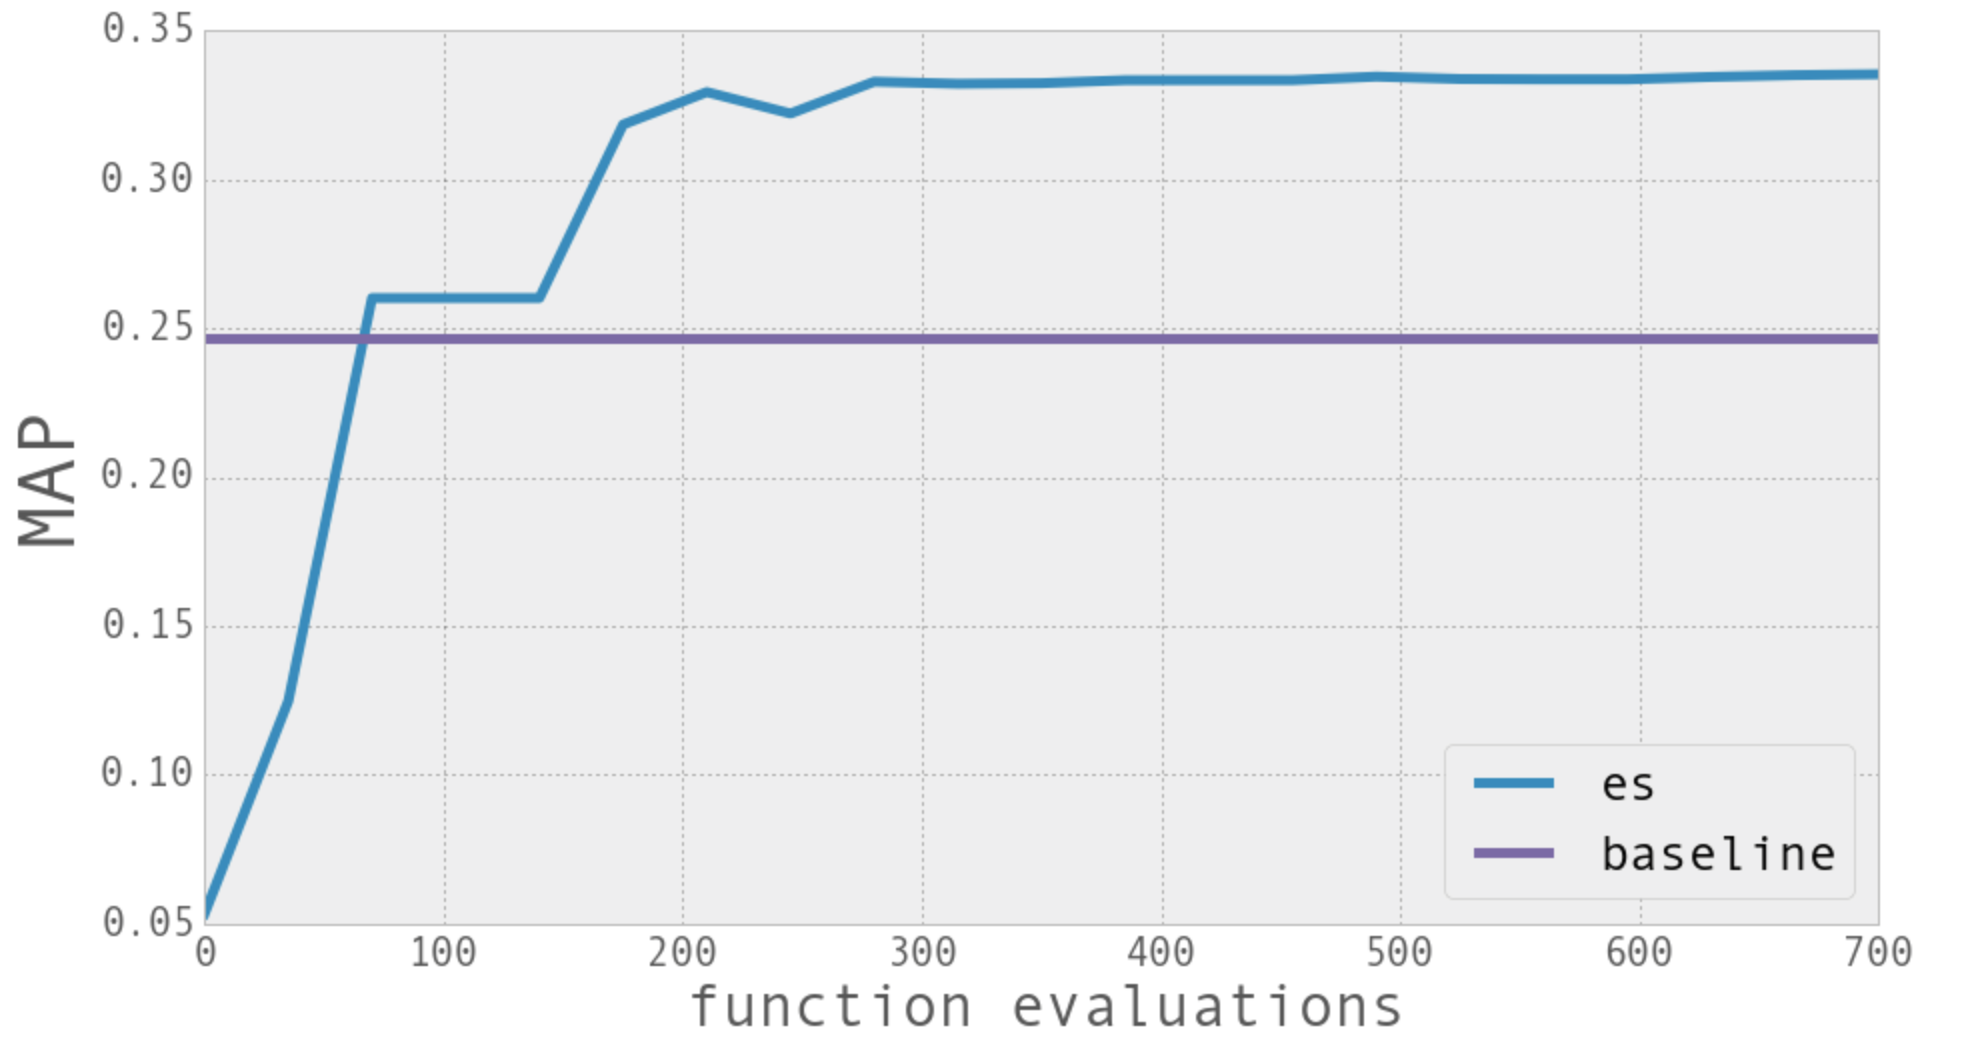
\includegraphics[width=0.75\textwidth]{figures/es_lab3.png}
		\caption{MAP durante ottimizzazione laboratorio 3.}
		\label{fig:es_lab3}
	\end{center}
\end{figure}
\begin{figure}[htbp]
	\begin{center}
		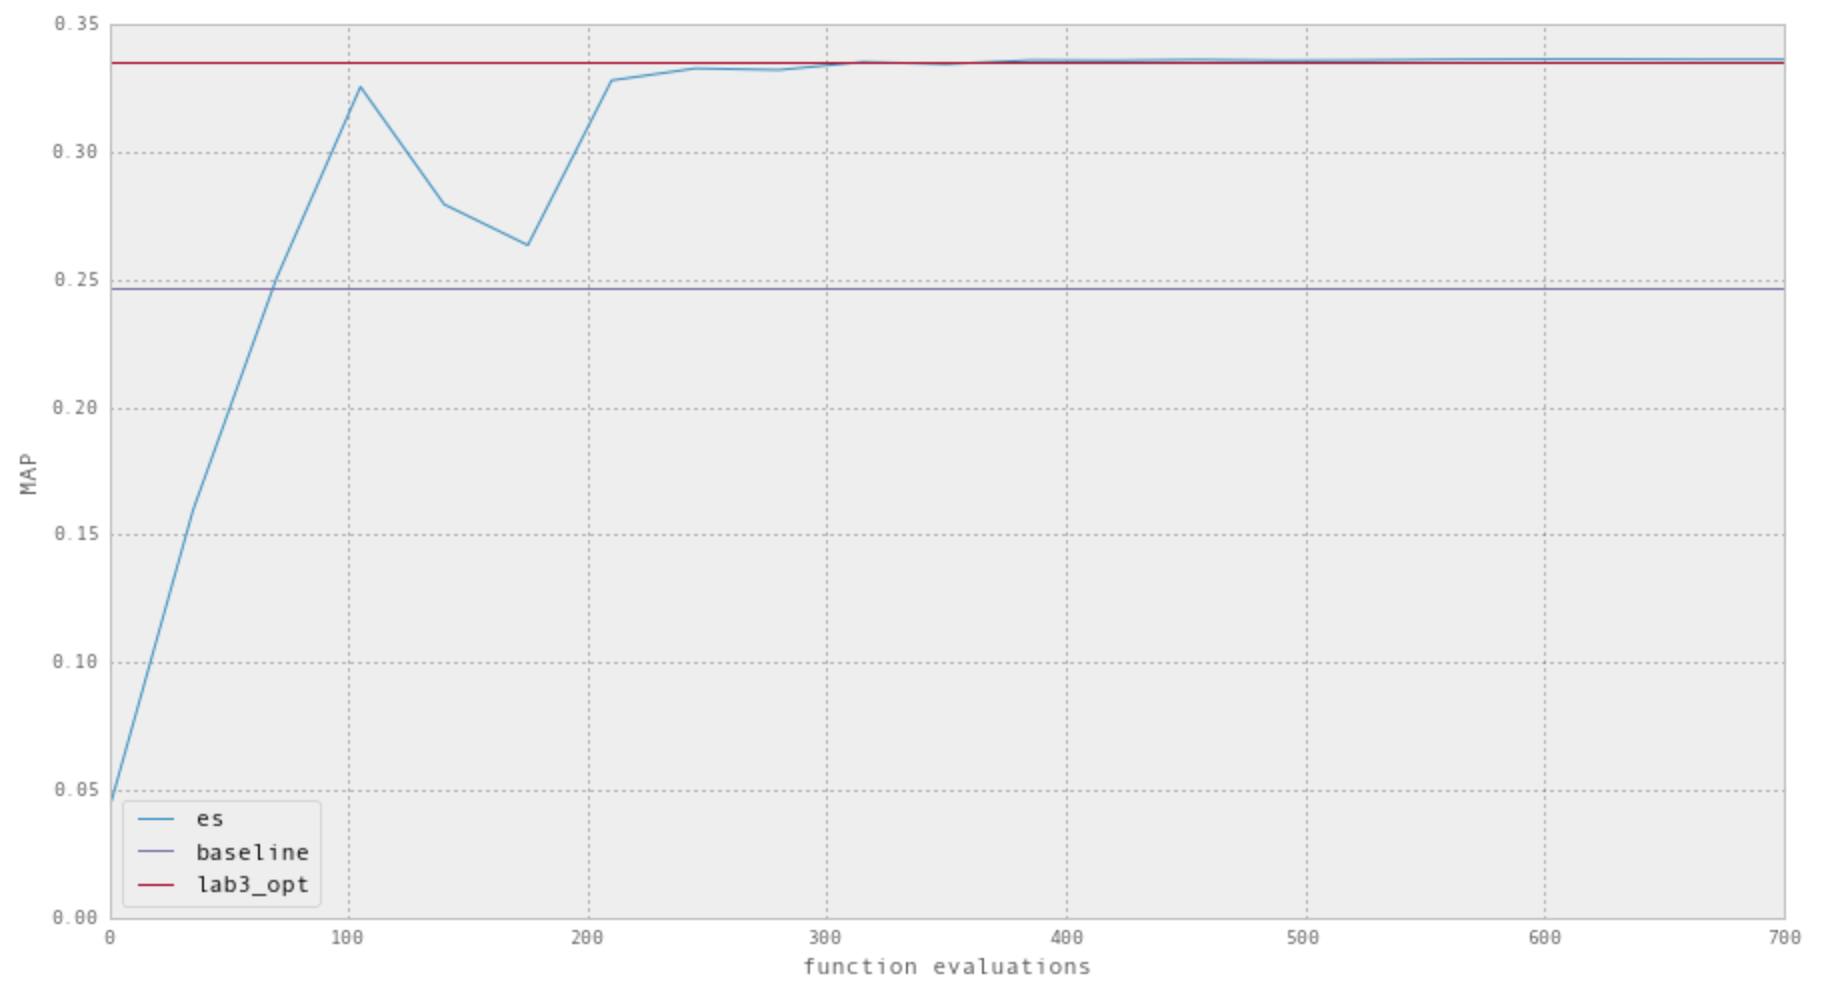
\includegraphics[width=0.75\textwidth]{figures/es_lab5.png}
		\caption{MAP durante ottimizzazione laboratorio 5.}
		\label{fig:es_lab5}
	\end{center}
\end{figure}
\begin{figure}[htbp]
	\begin{center}
		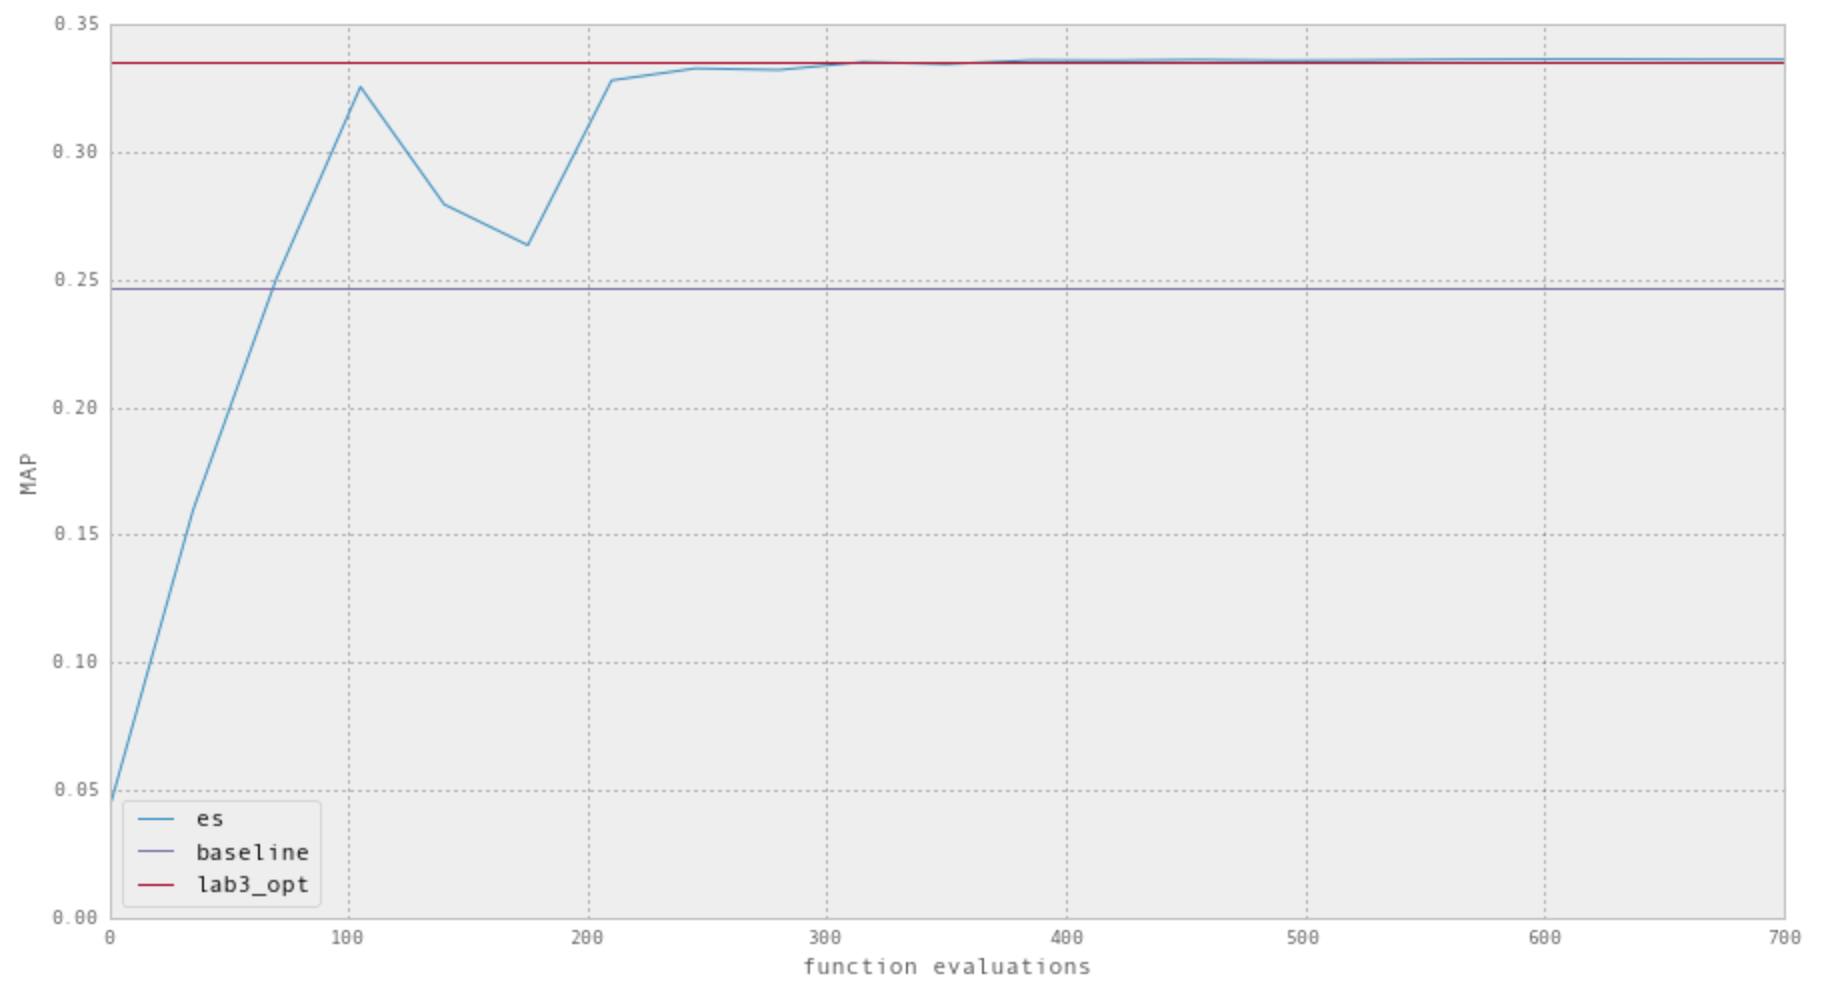
\includegraphics[width=0.75\textwidth]{figures/es_lab5.png}
		\caption{MAP durante ottimizzazione laboratorio 7.}
		\label{fig:es_lab7}
	\end{center}
\end{figure}

Tabella \ref{tab:es} riporta i risultati dell'ottimizzazione.
\begin{table}[htdp]
\caption{Risultati ottimizzazione con ES per i vari laboratori.}
\begin{center}
\begin{tabular}{|c|c|c|}
\hline
laboratorio & parametri & MAP \\
 \hline
3 & $k_1 = 0.0253, b = 0.0221$ & $0.3354$ \\
5 & $k_1 = 0.0237, b = 0.0, \alpha=0.7832$ & $0.3366$ \\
7 & $k_1 = 0.0237, b = 0.0, \alpha=0.7832$ & $0.3366$ \\
\hline
\end{tabular}
\end{center}
\label{tab:es}
\end{table}

Come si puo' vedere grazie all'ES si e' ottenuto un notevole miglioramento in termini di MAP rispetto alla nostra prima versione. I risultati dell'ottimizzazione vengono discussi in Sezione \ref{sec:risult-sper}.

\subsection{Altri metodi}
tipo lucene
\label{sec:altri-metodi}

Se sono stati sviluppati altri metodi, descriverli qui.

